%\newcommand{\spcen}{\centering \vskip 0.05in}

\begin{table}[tbp]
%\footnotesize
\centering
\caption{\tabletitle{HIS}{Onemax}}
%\vskip 0.05in
\begin{tabular}{|r|r|rr|rr|}
\hline
\multicolumn{1}{|c|}{Samples} & \multicolumn{1}{c|}{Cutoff} &
 \multicolumn{2}{c|}{Best} & 
 \multicolumn{2}{c|}{Evaluations}  \\ \hline
10 & 10 & --400 &  (0) & 29155 &  (12095.51) \\ \hline
10 & 20 & --400 &  (0) & 32743 &  (11000.43) \\ \hline
50 & 10 & --400 &  (0) & 48435 &  (20868.97) \\ \hline
10 & 30 & --400 &  (0) & 56170 &  (16627.74) \\ \hline
10 & 40 & --400 &  (0) & 67595 &  (20897.39) \\ \hline
50 & 20 & --400 &  (0) & 82215 &  (15277.81) \\ \hline
50 & 30 & --400 &  (0) & 113680 &  (23360.03) \\ \hline
50 & 40 & --400 &  (0) & 157715 &  (35272.9) \\ \hline
\end{tabular}
\label{his-onemax}
\end{table}

\begin{figure}[tbp]
\centering
\centerline{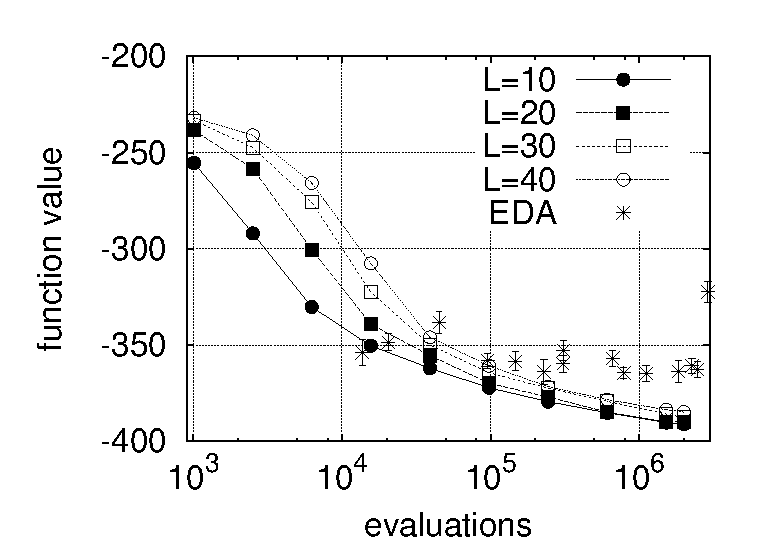
\includegraphics[width=\figlength\linewidth]{./data_his/his_1dising_s10.eps}}
(a) $M=10$\\
\vspace{0.1in}
\centerline{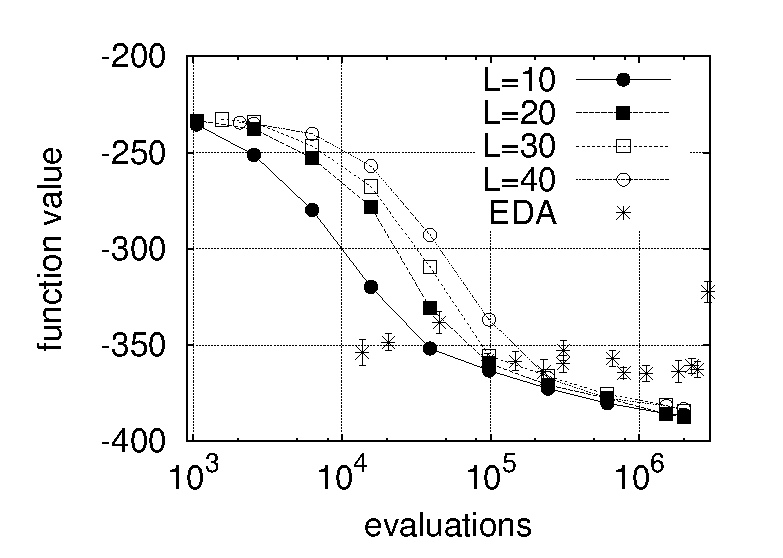
\includegraphics[width=\figlength\linewidth]{./data_his/his_1dising_s50.eps}}
(b) $M=50$
\caption{\tabletitle{HIS}{1D Ising}}
\label{his-1d-ising}
\end{figure}

\begin{figure}
\centering
\centerline{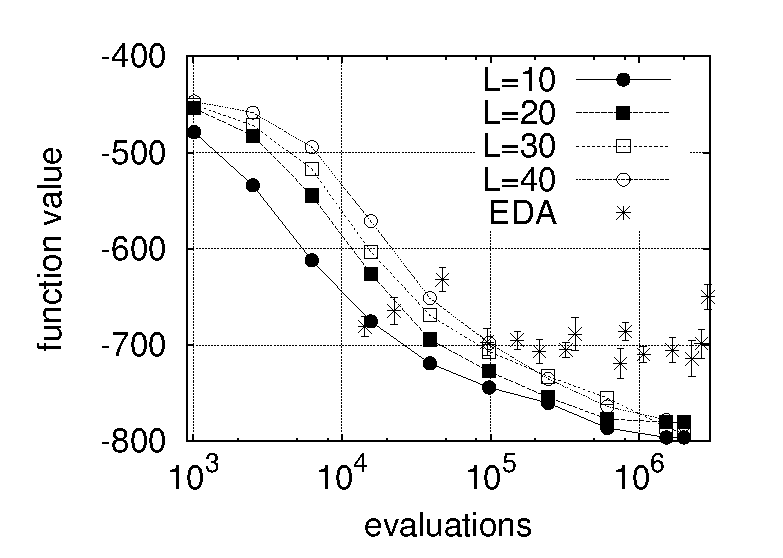
\includegraphics[width=\figlength\linewidth]{./data_his/his_2dising_s10.eps}}
(a) $M=10$ \\
\vspace{0.1in}
\centerline{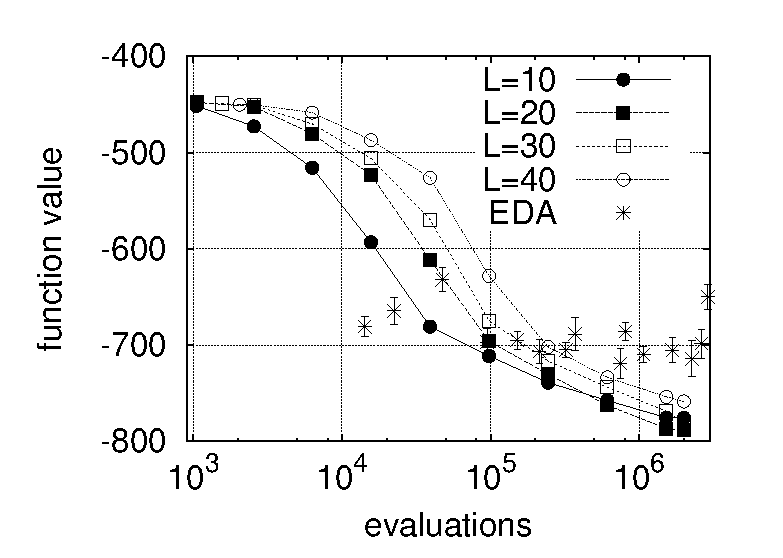
\includegraphics[width=\figlength\linewidth]{./data_his/his_2dising_s50.eps}}
(b) $M=50$
\caption{\tabletitle{HIS}{2D Ising}}
\label{his-2d-ising}
\end{figure}

%\vskip 0.2in

